\begin{figure}
\centering
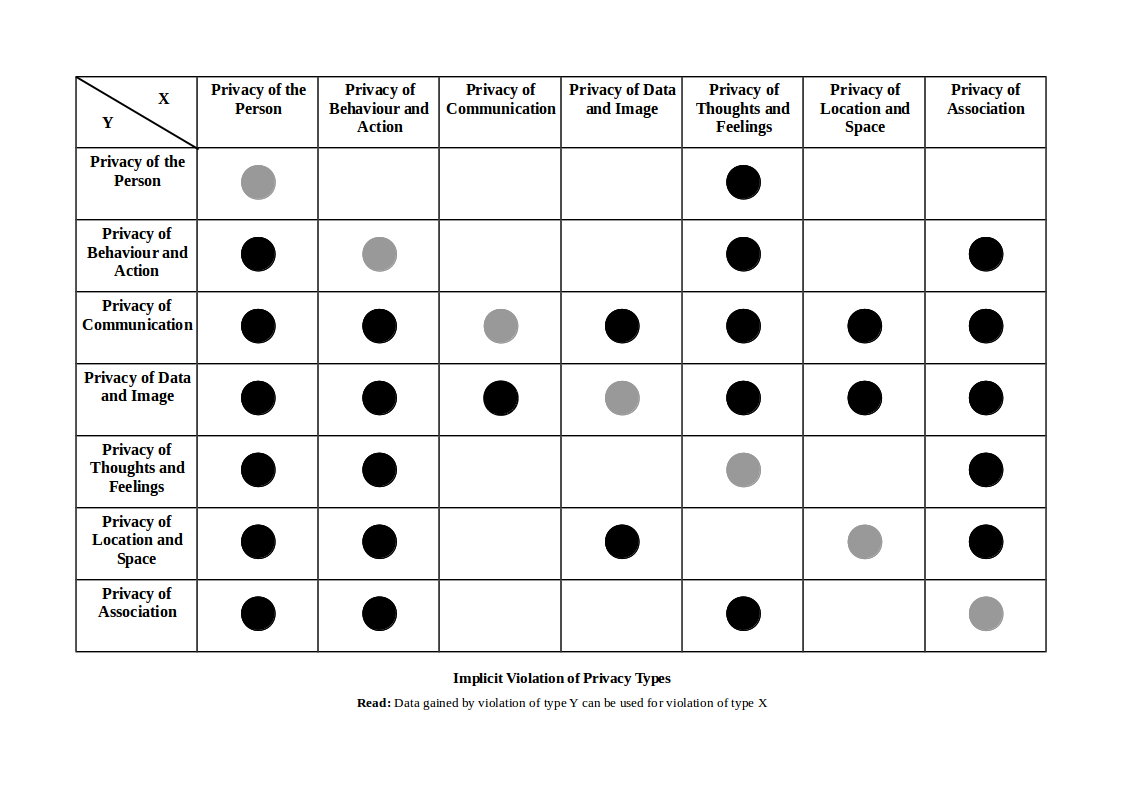
\includegraphics{diagrams/png/implicit-privacy-violation-matrix.png}

\begin{flushleft}
\scriptsize
\textbf{Legend:}
The matrix above shows the following relation: \emph{Type X can be
implicitly violated by the violation of type Y.}
\begin{itemize}
\itemsep1pt\parskip0pt\parsep0pt
\item
  The X-Axis shows the Seven Types of Privacy according to Friedewald et
  al., which could be violated implicitly
\item
  The Y-Axis shows the Seven Types of Privacy according to Friedewald et
  al., which have been violated explicitly
\item
  Big black bullet points denote, that an implicit violation is possible
\item
  Big grey bullet points only denote, that the relation is reflexive
  (\emph{a R a}). They are only shown for completeness sake and not
  discussed further, because they denote a trivial fact.
\end{itemize}
\end{flushleft}

\caption{Implicit Privacy Violation Matrix}
\label{figure:Implicit Privacy Violation Matrix}
\end{figure}
